\documentclass{../ucll-slides}
\usepackage{../pvm}
\usetikzlibrary{shadows,shapes.multipart}

\title{Preprocessor}
\author{Fr\'ed\'eric Vogels}



\begin{document}

\begin{frame}
  \titlepage
\end{frame}

\begin{frame}
  \frametitle{Problem Statement}
  \begin{itemize}
    \item We've discussed forward declarations
    \item Forward declarations specify type information
    \item Compiler needs to keep this information in memory
    \item Large programs have large number of functions/classes
    \item Compiler can't fit all this data in memory
  \end{itemize}
\end{frame}

\begin{frame}
  \frametitle{Solution}
  \begin{itemize}
    \item Divide the codebase in small units
    \item ``Compilation units'' (CUs): {\tt .cpp} files
    \item In each file we put the minimal amount of declarations
    \item Compile each unit separately
    \item Link results together
  \end{itemize}
\end{frame}

\begin{frame}
  \frametitle{Build Steps}

  \begin{center}
    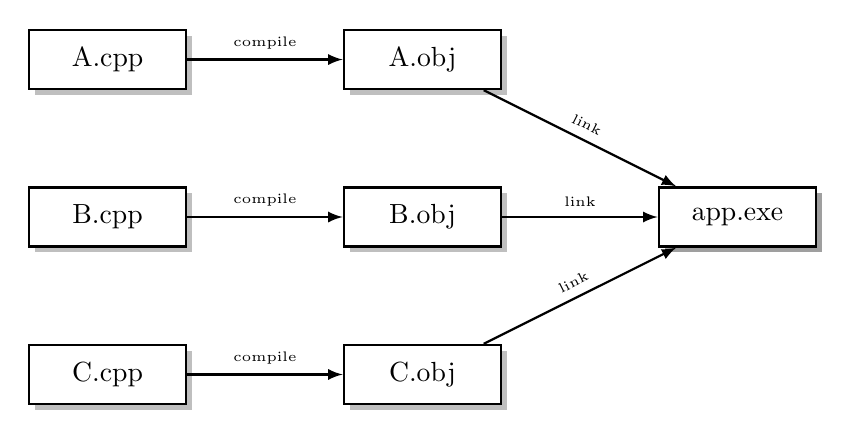
\begin{tikzpicture}[cpp/.style={draw,thick,drop shadow,fill=white,minimum width=2cm,minimum height=.75cm},
                        obj/.style={draw,thick,drop shadow,fill=white,minimum width=2cm,minimum height=.75cm},
                        exe/.style={draw,thick,drop shadow,fill=white,minimum width=2cm,minimum height=.75cm},
                        compile/.style={-latex,thick},
                        compile arc/.style={above,midway,font=\tiny},
                        link/.style={-latex,thick},
                        link arc/.style={above,midway,font=\tiny,sloped}]
      \node[cpp] (a cpp) at (0,4) {A.cpp};
      \node[cpp] (b cpp) at (0,2) {B.cpp};
      \node[cpp] (c cpp) at (0,0) {C.cpp};

      \visible<2->{
        \node[obj] (a obj) at (4,4) {A.obj};
      }

      \visible<2>{
        \draw[compile] (a cpp) -- (a obj) node[compile arc] {compile};
      }

      \visible<3->{
        \node[obj] (b obj) at (4,2) {B.obj};
      }

      \visible<3>{
        \draw[compile] (b cpp) -- (b obj) node[compile arc] {compile};
      }

      \visible<4->{
        \node[obj] (c obj) at (4,0) {C.obj};
      }

      \visible<4>{
        \draw[compile] (c cpp) -- (c obj) node[compile arc] {compile};
      }
      
      \visible<5->{
        \node[exe] (exe) at (8,2) {app.exe};
      }
      
      \visible<5>{
        \node[exe] (exe) at (8,2) {app.exe};
        \draw[link] (a obj) -- (exe) node[link arc] {link};
        \draw[link] (b obj) -- (exe) node[link arc] {link};
        \draw[link] (c obj) -- (exe) node[link arc] {link};
      }
    \end{tikzpicture}
  \end{center}
\end{frame}

\begin{frame}
  \frametitle{Example}
  \code[width=10cm,title={App.cpp},frame=lines]{ex1.cpp}
\end{frame}

\begin{frame}
  \frametitle{Example}
  \code[width=10cm,title={App.cpp},frame=lines]{ex1-decl.cpp}
\end{frame}

\begin{frame}
  \frametitle{Example}
  \code[width=10cm,title={foo.cpp},frame=lines]{ex1-foo.cpp}
  \code[width=10cm,title={bar.cpp},frame=lines]{ex1-bar.cpp}
  \code[width=10cm,title={qux.cpp},frame=lines]{ex1-qux.cpp}
\end{frame}

\begin{frame}
  \frametitle{Example}
  \begin{itemize}
    \item Each file can be compiled separately
    \item Each file contains minimal but sufficient declarations
  \end{itemize}
  \code[width=3cm]{decl.cpp}
  \begin{center}
    means \\[7mm]
    ``Some function {\tt foo} exists. It has one parameter of type {\tt int},
    and returns a {\tt bool}. If you do not encounter it in this file,
    I promise you you will find it in another one.''
  \end{center}
\end{frame}

\begin{frame}
  \frametitle{Linker}
  \begin{itemize}
    \item The compiler will believe your promises
    \item If you do not \emph{define} your declared function,
          compiler will assume it's in some other CU
    \item Linker is less naive
    \item Linker will check promises
    \item Missing \emph{definition} will lead to linker error
  \end{itemize}
\end{frame}

\begin{frame}
  \frametitle{Engineering Nightmare}
  \begin{center}
    \begin{tikzpicture}[definition/.style={fill=red!50,draw,rectangle split,rectangle split parts=2},
                        declaration/.style={fill=blue!50,draw,rectangle split,rectangle split parts=2},
                        reference/.style={-latex}]
      \node[definition] (definition) at (0,0) {
        def.cpp
        \nodepart{two}
        \tt void \only<1>{foo}\only<2->{{\color{red} bar}}() \{ \dots\ \}
      };

      \foreach[count=\i] \x in {0,60,...,300} {
        \node[declaration] (declaration \i) at (\x:3.5) {
          file\i.cpp
          \nodepart{two}
          \tikzmath{
            int \j;
            int \k;
            \j = int(\i + 1);
            \k = int(\j + 1);
          }
          \tt void \only<1-\j>{foo}\only<\k->{{\color{red}bar}}();
        };
        \draw[reference] (declaration \i) -- (definition);
      }
    \end{tikzpicture}
  \end{center}
\end{frame}

\begin{frame}
  \frametitle{Engineering Nightmare}
  \begin{itemize}
    \item Say the definition changes
          \begin{itemize}
            \item Name change
            \item Parameter change
            \item Return type change
          \end{itemize}
    \item Then all CUs containing a declaration need to be updated
    \item Due to redundancy: same declaration in many files
  \end{itemize}
\end{frame}

\begin{frame}
  \frametitle{Engineering Nightmare}
  \begin{itemize}
    \item Say the definition changes
          \begin{itemize}
            \item Name change
            \item Parameter change
            \item Return type change
          \end{itemize}
    \item Then all CUs containing a declaration need to be updated
    \item Due to redundancy: same declaration in many files
  \end{itemize}
\end{frame}

\begin{frame}
  \frametitle{Solution}
  \begin{itemize}
    \item Make {\tt cpp} file responsible for generating a list of declarations
          for all of its definitions
    \item Put these declarations in separate file
    \item Include the contents of this ``twin'' file in other {\tt cpp} files
    \item This ``twin'' file is called a \emph{header file}
  \end{itemize}
\end{frame}

\begin{frame}
  \frametitle{Header Files}
  \begin{columns}[t]
    \column{5cm}
    \code[width=5cm,title={funcs.cpp},frame=lines]{cpp-file.cpp}
    \column{5cm}
    \code[width=5cm,title={funcs.h},frame=lines]{header-file.h}
  \end{columns}
\end{frame}

\begin{frame}
  \frametitle{Including Header Files}
  \code[title={main.cpp},frame=lines,width=5cm]{including.cpp}
\end{frame}

\begin{frame}
  \frametitle{Visualisation}
  \begin{center}
    \begin{tikzpicture}[cpp/.style={fill=red!50,draw},
                        h/.style={fill=blue!50,draw},
                        includes/.style={-latex}]
      \foreach[count=\i] \x in {0,120,240} {
        \tikzmath{
          real \y;
          \y = \x + 90;
        }

        \node[cpp,rotate=\y] (file \i) at (\x:3) {
          file\i.cpp
        };

        \node[h,rotate=\y] (header \i) at (\x:2) {
          file\i.h
        };

        \draw[includes] (file \i) -- (header \i);
      }

      \draw[includes] (file 1) -- (header 2);
      \draw[includes] (file 2) -- (header 3);
      \draw[includes] (file 3) -- (header 1);

      \draw[includes] (file 1) -- (header 3);
      \draw[includes] (file 2) -- (header 1);
      \draw[includes] (file 3) -- (header 2);
    \end{tikzpicture}
  \end{center}
\end{frame}

\begin{frame}
  \frametitle{Typical Structure of {\tt cpp} file}
  \code[title={file.cpp},frame=lines]{header-example.cpp}
  \begin{itemize}
    \item First include: preferably own header file
    \item What's the reason for this? \cake
  \end{itemize}
\end{frame}

\begin{frame}
  \frametitle{Preprocessor}
  \begin{itemize}
    \item {\tt \#include} is a preprocessor directive
    \item Preprocessor is a separate minilanguage
    \item All code gets processed by the preprocessor first
  \end{itemize}
  \vskip4mm
  \begin{center}
    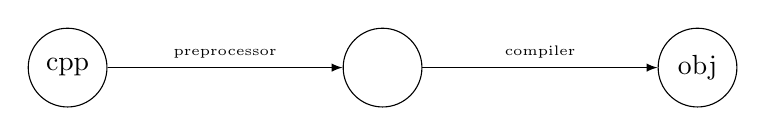
\begin{tikzpicture}[file/.style={circle,minimum size=1cm,draw},
                        translate/.style={-latex}]
      \node[file] (cpp) at (0,0) {cpp};
      \node[file] (intermediate) at (4,0) {};
      \node[file] (obj) at (8,0) {obj};

      \draw[translate] (cpp) -- (intermediate) node[midway,above,font=\tiny] {preprocessor};
      \draw[translate] (intermediate) -- (obj) node[midway,above,font=\tiny] {compiler};
    \end{tikzpicture}
  \end{center}
\end{frame}

\begin{frame}
  \frametitle{{\tt \#include Directive}}
  \begin{itemize}
    \item {\tt \#include "file"} is replaced by the contents of {\tt file}
    \item Works with \emph{any} file, on any line
    \item Preprocessor does not care about contents of files
  \end{itemize}
  \begin{columns}
    \column{5cm}
    \code[title={file.cpp},frame=lines,width=5cm]{include-example.cpp}
    \code[title={bla.txt},frame=lines,width=5cm]{bla.txt}
    \column{5cm}
    \code[title=result,frame=lines,width=5cm]{include-result.cpp}
  \end{columns}
\end{frame}

\begin{frame}
  \frametitle{Problem: Headers With Dependencies}
  \begin{center}
    \begin{tikzpicture}[file/.style={rectangle split,rectangle split parts=2,draw},
                        cpp/.style={file,fill=red!50},
                        h/.style={file,fill=blue!50},
                        includes/.style={-latex}]
      \node[cpp] (C cpp) at (0,0) {
        {\tt C.cpp}
        \nodepart{two}
        def.\ class {\tt C}
      };

      \node[h,anchor=north] (C h) at ($ (C cpp.south) + (0,-.5) $) {
        {\tt C.h}
        \nodepart{two}
        decl.\ class {\tt C}
      };

      \node[cpp] (foo cpp) at (4,0) {
        {\tt foo.cpp}
        \nodepart{two}
        void foo(C c) { \dots }
      };

      \node[h,anchor=north] (foo h) at ($ (foo cpp.south) + (0,-.5) $) {
        {\tt foo.h}
        \nodepart{two}
        void foo(C);
      };

      \node[cpp] (bar cpp) at (8,0) {
        {\tt bar.cpp}
        \nodepart{two}
        uses foo
      };

      \draw[includes] (C cpp) -- (C h);
      \draw[includes] (foo cpp) -- (foo h);
      \draw[includes] (foo cpp) -- (C h);
      \draw[includes] (bar cpp) -- (foo h);
    \end{tikzpicture}
  \end{center}
\end{frame}

\begin{frame}
  \frametitle{Problem: Headers With Dependencies}
  \begin{overprint}
    \onslide<1>
    \code[title=bar.cpp,frame=lines]{header-dependencies1.cpp}
    \onslide<2->
    \code[title=bar.cpp,frame=lines]{header-dependencies2.cpp}
  \end{overprint}
  \visible<3>{
    \begin{center}
      Compiler doesn't know type {\tt C}!
    \end{center}
  }
\end{frame}

\begin{frame}
  \frametitle{Proposed Solution \#1}
  \code[title=bar.cpp,frame=lines]{header-dependencies3.cpp}
  \begin{itemize}
    \item Have {\tt bar.cpp} also include {\tt C.h}
    \item Include order important $\rightarrow$ fragile
    \item Does {\tt bar.cpp} need to know of {\tt foo.h}'s dependency?
    \item If header file gets extra dependencies, all including {cpp} files
          would need to be updated
    \item Again, engineering nightmare
  \end{itemize}  
\end{frame}

\begin{frame}
  \frametitle{Proposed Solution \#2}
  \begin{overprint}
    \onslide<1>
    \code[title=bar.cpp,frame=lines]{header-dependencies4.cpp}
    \code[title=foo.h,frame=lines]{header-dependencies4-foo.h}
    \onslide<2>
    \code[title=bar.cpp,frame=lines]{header-dependencies5.cpp}
    \onslide<3>
    \code[title=bar.cpp,frame=lines]{header-dependencies6.cpp}
  \end{overprint}
  \begin{itemize}
    \item Have {\tt foo.h} include {\tt C.h}
  \end{itemize}
\end{frame}

\begin{frame}
  \frametitle{Visualisation Solution \#2}
  \begin{center}
    \begin{tikzpicture}[file/.style={rectangle split,rectangle split parts=2,draw},
                        cpp/.style={file,fill=red!50},
                        h/.style={file,fill=blue!50},
                        includes/.style={-latex}]
      \node[cpp] (C cpp) at (0,0) {
        {\tt C.cpp}
        \nodepart{two}
        def.\ class {\tt C}
      };

      \node[h,anchor=north] (C h) at ($ (C cpp.south) + (0,-.5) $) {
        {\tt C.h}
        \nodepart{two}
        decl.\ class {\tt C}
      };

      \node[cpp] (foo cpp) at (4,0) {
        {\tt foo.cpp}
        \nodepart{two}
        void foo(C c) { \dots }
      };

      \node[h,anchor=north] (foo h) at ($ (foo cpp.south) + (0,-.5) $) {
        {\tt foo.h}
        \nodepart{two}
        void foo(C);
      };

      \node[cpp] (bar cpp) at (8,0) {
        {\tt bar.cpp}
        \nodepart{two}
        uses foo
      };

      \draw[includes] (C cpp) -- (C h);
      \draw[includes] (foo cpp) -- (foo h);
      \draw[includes,thick,red,dashed] (foo cpp) -- (C h);
      \draw[includes] (bar cpp) -- (foo h);
      \draw[includes,thick,green!50!black] (foo h) -- (C h);
    \end{tikzpicture}
  \end{center}
  \begin{itemize}
    \item The green arrow replaces the red one
  \end{itemize}
\end{frame}

\begin{frame}
  \frametitle{Rules of Thumb}
  \begin{itemize}
    \item {\tt X.cpp} includes its own header file {\tt X.h} first
    \item {\tt X.h} includes minimal but sufficient selection of header files
      \begin{itemize}
        \item Litmus test: a {\tt cpp} with only {\tt \#include "X.h"} must compile
      \end{itemize}
    \item Let {\tt X.cpp} include all extra header files it needs
  \end{itemize}
\end{frame}

\begin{frame}
  \frametitle{Standard Library}
  \begin{itemize}
    \item Standard \cpp\ library accessible through header files
    \item Including using {\tt < >} instead of {\tt " "}
    \item {\tt < >} looks for header files in different place (\link{http://www.open-std.org/JTC1/SC22/WG14/www/docs/n1256.pdf}{C 6.10.2/2-3})
    \item C libraries: header files end in {\tt .h}
    \item \cpp\ libraries: header files without extension
    \item Strings: {\tt \#include <string>}
    \item Vector: {\tt \#include <vector>}
    \item IO streams: {\tt \#include <iostream>}
    \item \dots
    \item Best to include them last \cake
  \end{itemize}
\end{frame}

\begin{frame}
  \frametitle{New Problem: Multiply Included Header Files}
  \begin{center}
    \begin{tikzpicture}[file/.style={rectangle split,rectangle split parts=2,draw},
                        cpp/.style={file,fill=red!50},
                        h/.style={file,fill=blue!50},
                        includes/.style={-latex}]
      \node[cpp] (C cpp) at (0,0) {
        {\tt C.cpp}
        \nodepart{two}
        \parbox{3cm}{\tt
          \#include "C.h" \\
          \#include "D.h"
        }
      };

      \node[h,anchor=north] (C h) at ($ (C cpp.south) + (-2,-1) $) {
        {\tt C.h}
        \nodepart{two}
        {\tt \#include "X.h"}
      };

      \node[h,anchor=north] (D h) at ($ (C cpp.south) + (2,-1) $) {
        {\tt D.h}
        \nodepart{two}
        {\tt \#include "X.h"}
      };

      \node[h,anchor=north] (X h) at ($ (C cpp.south) + (0,-3) $) {
        {\tt X.h}
        \nodepart{two}
        {\tt ...}
      };

      \draw[includes] (C cpp) -- (C h);
      \draw[includes] (C cpp) -- (D h);
      \draw[includes] (C h) -- (X h);
      \draw[includes] (D h) -- (X h);
    \end{tikzpicture}
    \vskip5mm
    {\tt X.h} included twice!
  \end{center}
\end{frame}

\begin{frame}
  \frametitle{New Problem: Multiply Included Header Files}
  \begin{itemize}
    \item It's easy for situations to occur where the same header
          files gets included multiple times (typically with headers from
          the standard \cpp\ library)
    \item Is this bad? It depends on what the header file contains
    \item Multiple declarations in same compilation unit: ok
    \item Other stuff: only allowed once
    \item We need a way to prevent multiple includes
  \end{itemize}
\end{frame}

\begin{frame}
  \frametitle{Solution: Preprocessor Macros}
  \code[title=X.h,frame=lines,width=5cm]{include-guard.h}
  \begin{itemize}
    \item Initially {\tt X\_H\_INCLUDED} is not defined
    \item First include: the {\tt \#if} condition is true
    \item {\tt X\_H\_INCLUDED} gets defined
    \item Second include: {\tt X\_H\_INCLUDED} is defined
    \item Preprocessor leaves out contents of header file
  \end{itemize}
\end{frame}

\begin{frame}
  \frametitle{Example}
  \begin{columns}[t]
    \column{5cm}
    \begin{center} Before preprocessing \end{center}
    \code[title=X.h,frame=lines,width=5cm]{include-guard-example.h}
    \code[title=X.cpp,frame=lines,width=5cm]{include-guard-example2.h}
    \column{5cm}
    \begin{center} After preprocessing \\ (what the compiler sees) \end{center}
    \vskip2cm
    \code[frame=lines,width=5cm]{include-guard-example3.h}
  \end{columns}
\end{frame}

\begin{frame}
  \frametitle{Summary}
  \begin{columns}
    \column{6cm}
    \code[title=X.cpp,frame=lines,font size=\small]{summary.cpp}
    \column{6cm}
    \code[title=X.h,frame=lines,font size=\small]{summary.h}
  \end{columns}
\end{frame}

\begin{frame}
  \frametitle{More Macros}
  \begin{itemize}
    \item A macro is like a variable
          that can either be defined or undefined
    \item {\tt \#define {\it IDENTIFIER}}
    \item {\tt \#undef {\it IDENTIFIER}}
    \item {\tt \#ifdef {\it IDENTIFIER} ... \#endif}
    \item {\tt \#ifndef {\it IDENTIFIER} ... \#endif}
    \item {\tt \#ifdef {\it IDENTIFIER} ... \#else ... \#endif}
    \item {\tt \#ifndef {\it IDENTIFIER} ... \#else ... \#endif}
  \end{itemize}
\end{frame}

\begin{frame}
  \frametitle{More Macros}
  \begin{itemize}
    \item You can also use macros to define constants
  \end{itemize}
  \begin{columns}[t]
    \column{5cm}
    \begin{center} Before preprocessing \end{center}
    \code[font size=\small,frame=lines,width=5cm]{constant.cpp}
    \column{5cm}
    \begin{center} After preprocessing \\ (what the compiler sees) \end{center}
    \code[font size=\small,frame=lines,width=5cm]{constant-result.cpp}
  \end{columns}
\end{frame}

\begin{frame}
  \frametitle{More Macros}
  \begin{itemize}
    \item Macros can also behave function-like
  \end{itemize}
  \begin{overprint}
    \onslide<1>
    \code[font size=\small,frame=lines,title=Before preprocessing]{nullcheck.cpp}
    \onslide<2>
    \code[font size=\small,frame=lines,title=After preprocessing]{nullcheck-result.cpp}
  \end{overprint}
\end{frame}

\begin{frame}
  \frametitle{More Macros}
  \begin{itemize}
    \item Can be useful to introduce new syntax
    \item {\tt for} can be seen as a macro for {\tt while}, etc.
  \end{itemize}
  \begin{overprint}
    \onslide<1>
    \code[font size=\small,frame=lines,title=Before preprocessing]{forrange.cpp}
    \onslide<2>
    \code[font size=\small,frame=lines,title=After preprocessing]{forrange-result.cpp}
  \end{overprint}
\end{frame}

\begin{frame}
  \frametitle{More Macros}
  \begin{itemize}
    \item {\tt \#} can be used to stringify tokens
    \item More robust since less duplication necessary
  \end{itemize}
  \begin{overprint}
    \onslide<1>
    \code[font size=\small,frame=lines,title=Before preprocessing]{nullcheck2.cpp}
    \onslide<2>
    \code[font size=\small,frame=lines,title=After preprocessing]{nullcheck2-result.cpp}
  \end{overprint}
\end{frame}

\begin{frame}
  \frametitle{More Macros}
  \begin{itemize}
    \item {\tt \#} can be used to stringify tokens
    \item More robust since less duplication necessary
  \end{itemize}
  \begin{overprint}
    \onslide<1>
    \code[font size=\small,frame=lines,title=Before preprocessing]{nullcheck2.cpp}
    \onslide<2>
    \code[font size=\small,frame=lines,title=After preprocessing]{nullcheck2-result.cpp}
  \end{overprint}
\end{frame}

\begin{frame}
  \frametitle{More Macros: Predefined Macros}
  \begin{itemize}
    \item {\tt \_\_FILE\_\_}: containing file
    \item {\tt \_\_LINE\_\_}: line number on which this macro appears
    \item {\tt \_\_DATE\_\_}: date on which the preprocessor is being run
    \item {\tt \_\_TIME\_\_}: time at which the preprocessor is being run
  \end{itemize}
  \begin{overprint}
    \onslide<1>
    \code[font size=\small,frame=lines,title=Before preprocessing]{nullcheck3.cpp}
    \onslide<2>
    \code[font size=\small,frame=lines,title=After preprocessing]{nullcheck3-result.cpp}
  \end{overprint}
\end{frame}

\begin{frame}
  \frametitle{More Macros: Dangers}
  \begin{center}
    What could possibly go wrong?
  \end{center}
  \vskip1cm
  \begin{overprint}
    \onslide<1>
    \code[font size=\small,frame=lines,title=Before preprocessing]{min1.cpp}
    \onslide<2>
    \code[font size=\small,frame=lines,title=After preprocessing]{min2.cpp}
  \end{overprint}
\end{frame}

\begin{frame}
  \frametitle{More Macros: Dangers}
  \structure{Pros of {\tt min} as macro}
  \begin{itemize}
    \item Faster? No function call required!
    \item<2> Not faster! Functions can be inlined by compiler!
  \end{itemize}
  \vskip4mm
  \structure{Cons of {\tt min} as macro}
  \begin{itemize}
    \item Doesn't behave like regular functions
    \item Surprising behaviour
  \end{itemize}
\end{frame}

\begin{frame}
  \frametitle{Important Usage: Debug and Release Builds}
  \code[font size=\small]{assert.cpp}
  \begin{itemize}
    \item {\tt assert} macro to check assumptions
    \item Comes in very handy in  \cpp
    \item While debugging: define {\tt DEBUGGING}
    \item For performance: don't define {\tt DEBUGGING}
    \item Easy way to turn on/off diagnostic code
  \end{itemize}
\end{frame}

\begin{frame}
  \frametitle{Debug and Release Builds}
  \begin{itemize}
    \item Debug and Release builds generally known by IDE
    \item Release build: {\tt NDEBUG} is defined
    \item {\tt assert} already defined for you
  \end{itemize}
  \code[width=5cm]{include-assert.cpp}
\end{frame}

\end{document}